% Created 2015-05-18 Mon 01:15
\documentclass[9pt,b5paper]{article}
\usepackage{graphicx}
\usepackage{xcolor}
\usepackage{xeCJK}
\setCJKmainfont{SimSun}
\usepackage{longtable}
\usepackage{float}
\usepackage{textcomp}
\usepackage{geometry}
\geometry{left=0cm,right=0cm,top=0cm,bottom=0cm}
\usepackage{multirow}
\usepackage{multicol}
\usepackage{listings}
\usepackage{algorithm}
\usepackage{algorithmic}
\usepackage{latexsym}
\usepackage{natbib}
\usepackage{fancyhdr}
\usepackage[xetex,colorlinks=true,CJKbookmarks=true,linkcolor=blue,urlcolor=blue,menucolor=blue]{hyperref}


\lstset{language=c++,numbers=left,numberstyle=\tiny,basicstyle=\ttfamily\small,tabsize=4,frame=none,escapeinside=``,extendedchars=false,keywordstyle=\color{blue!70},commentstyle=\color{red!55!green!55!blue!55!},rulesepcolor=\color{red!20!green!20!blue!20!}}
\author{deepwaterooo}
\date{\today}
\title{MIDI Command Controller Interface}
\hypersetup{
  pdfkeywords={},
  pdfsubject={},
  pdfcreator={Emacs 24.3.1 (Org mode 8.2.7c)}}
\begin{document}

\maketitle
\tableofcontents


\section{update 5/17/2015}
\label{sec-1}
\begin{itemize}
\item It's NOT necessary to separate the player into a separate thread, because QWidget subfamilies are NOT thread safe, I will still keep the phonon-related functions in the mainwindow main GUI, just separate the checking midi port tasks into a separate thread.
\item checkout an old version of commits, and continue to remove the unnecessary menu bar, and musictable, together with fix the bugs\ldots{}.
\item deleted some unnecessary codes to remove menubar \& musicTable;
\item modified timeLcd to display total time as well, referring to advisor's rule that "the more information the better".
\item may work on make upper-leffer corner buttons look slightly better than current now\ldots{}.
\end{itemize}
\section{update 5/15/2015}
\label{sec-2}
\begin{itemize}
\item The advisor met his other student instead, meeting got rescheduled to be on coming Monday.
\item I applied for graduation on time before 5/12/2015, right now I am still WAITING for department of Engineering to approve for my study plan.
\item The Study Plan was finally approved by College of Graduate Studies, will be waiting for the Office of the Rigistrar to continue updates.
\item But after busy contacting these days, I still failed to figure out how to remove the unnecessary one course from my Degree Audit "Study Plan Detail" list. The personile was going home, and having Monday off, so I could only get my Study Plan eventually fixed earliest by coming Tuesday, if things goes smoothly\textasciitilde{}!
\end{itemize}

\section{update 5/11/2015, Monday}
\label{sec-3}
\begin{itemize}
\item Realized that except that the thread checking midi port run() is running in a separate thread, all others are still within the GUI main thread
\begin{itemize}
\item The bottom layer user reconfiguration section has limited steps and executed fast, produce barely noticable block, doesn't affect by thread that much.
\item But the phonon median player, I think if I could separate it into an independend thread, and then communicate with other thread, this multi-threads design should significantly improve the GUI responsiveness and user experience.
\item I needs high-level architecture design, but feels like the advisor barely offer help for me from this perspective.
\item Will discuss with the advisor today to see his ideas.
\end{itemize}
\item Project handling related thinking
\begin{itemize}
\item This project has lasted too long already, but I have never be any person that tend to be late and delay, examples include I was top 2 student who successfully accomplished the Tic-Tac-Toe one-best-move-step lisp hw2 program (according to certain criterion) for CS210 (Programming Language) within my first month of new major study (\textbf{Sep 18, 2012}, the course instructor delayed the due time for 1 day because majority of the class has no clue where to start). The reasons that I am late now for this project includes: 
\begin{itemize}
\item Ever since RTOS (Real Time Operating System course), I began to realize that this advisor is NOT that into programming, as well as has some difficulty to explain concepts clear. And for courses after courses, as cs is a new major for me, I have suffered from this, and I had NEVER have enough confidence in the course instuctor, and my performance was significantly affected by this.
\item From my side, as an international student, I also have difficulty in understanding concepts, and have slightly foreighn language related affects.
\item For my education and project experience, it's more like with a great mentor or team member, I performs great; On the other hand, if the environment doesn't help, I become a poor guy with barely any production\ldots{}.
\item This project experience for me, is like my personal learning how to swim process after having been drowned almost to death when I was a kid. The whole process feels lonely and helpless, and I have to stuggle my own way out, which always made me rewind the internship season when a experienced mentor could always help test the knowledge points (for example, the first time repack my program into modules so that my programs could be reusable, python sys.path.append("\ldots{}.") \url{https://github.com/deepwaterooo/MyAutobiography} \textbf{part2\textunderscore deepwaterooo-Autobiography.pdf} section 8.29 ʵϰ(26) 8.30 ʵϰ(27) \textbf{page 48 \& 49})
\end{itemize}
\end{itemize}
\item Review and Project Remaaining problems
\begin{itemize}
\item The advisor concludes that the project is \textbf{petty much there}
\item Midi LED ON/OFF is NOT as responsive as we expected. 
\begin{itemize}
\item I have used ./midi$_{\text{read}}$$_{\text{write}}$/midi$_{\text{usb}}$$_{\text{write}}$$_{\text{onteOnOff}}$.cpp single program to test midi device LED ON/OFF as well, the performance is NOT stable.
\item The advisor suggested mutex protection for shared data write. So I have tried adding those mutex lock() unlock() back, but it doesn't seem to help at all.
\item The advisor concludes that it could be my programs-related reasons, could be midi device issues, and could also be midi-usb software problems.
\end{itemize}
\item Following:
\begin{itemize}
\item I am not that into midi LED ON/OFF responsiveness issues, but would rather pack my programs so that it has more thread and performs more responsive than it is right now. Considering all the work I have done already, the advisor agreed.
\item I will continuously work from today to Thursday 2-9 pm, but still scheduled a potential meeting time with advisor on \textbf{coming Friday, 5/15/2015 1pm} expecting to make some progress on threads communications.
\end{itemize}
\end{itemize}
\item Other graduation related: the university \textbf{web system} made a mess with my study plan, they are working on it to remove one couse in my study plan, which I have never added it into my study plan. There is no reason it should NOT process well.
\end{itemize}

\section{update 5/9/2015}
\label{sec-4}
\begin{itemize}
\item look into error msgs:
\begin{itemize}
\item (midiUI:5544): Gtk-CRITICAL **: IA\textunderscore \textunderscore gtk\textunderscore widget\textunderscore get\textunderscore direction: assertion 'GTK\textunderscore IS\textunderscore WIDGET (widget)' failed
\begin{itemize}
\item QObjects constructed without parent are owned by Qt instead of PyQt, this error is probably a result of the destructor being called twice when exiting.
\item Not completely fixed yet.
\end{itemize}
\item GStreamer-CRITICAL **: gst\textunderscore pad\textunderscore link\textunderscore full: assertion 'GST\textunderscore IS\textunderscore PAD (sinkpad)' failed
\end{itemize}
\end{itemize}

\section{update 5/8/2015}
\label{sec-5}
\begin{itemize}
\item add a configure file for latest user configuration for key-song bindings.
\item add a QFile read/write utility class. Default loading, user re-configuration, save to default are all fully functional for the bottom section now.
\item connected 33 "Browse" buttons with the 33 QPlainTextEdit editors through QSignalMapper, which I had applied similar connections one-by-one for Senior design for last semester!
\item Upper section Midi LED ON/OFF still needs focus and some work, will spend some hours continuously on it tomorrow.
\item Remove menubar and musicTable is the easiest thing to do, temporatorily keep them for debugging propose only.
\end{itemize}

\section{update 5/5/2015, Tuesday}
\label{sec-6}
\subsection{updates}
\label{sec-6-1}
\begin{itemize}
\item About the phonon playing, debugged and found out that my problem was only because I failed to point the correct complete path for .wav files, instead of only Song name without path.
\item Combined ReadFromMidi and WriteToMidi into one thread, and use "\textbf{volatile}".
\item Could paint the QPushButtons on and off from GUI responsively; Lighted midi LED on but afterwards failed, won't be difficult to solve.
\end{itemize}
\subsection{Detailed Requirements}
\label{sec-6-2}
\begin{itemize}
\item \textbf{Bottom configuration set up}, "all the GUI design has no problem, and keeps the same" (according to the advisor), but implement it so that the use could reconfigure the combining between midi command keys and the song it will play. The detail would be load the default or lasted saved configurations when software initialize from one separate file, and save all the used made configurations before close the software (so always keep one configuration file).
\item \textbf{Menu bar:} remove the menu bar as well discussed before. Don't need it;
\item \textbf{Midi Layout:} midi layout looks fine, and keep the same untouched;
\item \textbf{Music Table:} The advisor's basic rule keeps the same, "\textbf{the more information that better.}" So he want to keep the seekslider, LCD tiem ticks, volumeSlider, play/pause/stop action buttons, but remove the last two (first/last?), which were useless, and remove the musicTable from the GUI layout as well, becuase the currently playing song can be know from the QPushButton painted with color and the song name the QPushButton corresponded to from the bottom configuration part.
\end{itemize}

\subsection{Other}
\label{sec-6-3}
\begin{itemize}
\item My "\textbf{Change of Study Plan Form}" was sent out to the advisor through university email system more than one week ago, and I am still waiting for the advisor's approve. Check with him what's going on. 
\begin{itemize}
\item The advisor simply said that he justed didn't have time to look into it, will look into it during the next couple of days.
\item Suggested me submit my application for graduation at the same time.
\end{itemize}

\item Discuss Summer pan with the advisor today. 
\begin{itemize}
\item I will leave for CA Silleycon Valley next weekend (about ten days later), and I will still seek internship for professional practise and at the same time earn some money.
\item So I would want to finish and wrap up the whole project by next Friday.
\item The advisor said he has two tests during final week, so we planed to meet on \textbf{Monday 10:00am - 11:00am} next week targeted for project review (so that I would only worried about minor left parts during coming summer, when I should focus on my internship tasks.)
\end{itemize}

\item Continued with the project up to this point, my feeling was complicated, felt so sorry for the years I have spent here. will write them into words and update them after the review. 
\begin{itemize}
\item About three years ago in \textbf{Aug 2012}, when I have planed to go back to china (if I can select only \textbf{7 credits} for the first semester with \textbf{cs120 B} as the only background), the ex-advisor and the famous professor from the department made me stay by giving me permission to select more credits;
\item The famous professor from the department made me walk around many important courses, like algorithms, software engineering etc, without giving me any course opportunity to build any solid background, like kicked me off from cs480 so that I don't have to take cs481 for Spring 2015, such that they -- the department doesn't have to give me a TA for the spring semester after I have paid self-supported tuition fees continuously for three semesters \ldots{} After five semesters hard work and good performance, eventually I still have to do labor work to make a living here on campus \ldots{}.
\item The famous professor from the department designed the uncooperate character for me by having asked me to change advisor when we don't have much conflicts at that time yet\ldots{} I have worked in the same company in 2010 and 2011 for Nielson Online twice. Cooperative or Uncooperative, it has been more a policy or U.S.A. culture towards me now instead of my own character/personality !
\item It's painful to rewind back all these bad memory and details. I will continuously update this part later when I get my mind back systematically.
\end{itemize}

\item Saw the advisor in main office, should be here shortly. 
\begin{itemize}
\item The advisor showed up in CSAC at around 10:14am, but talked to somebody else until 10:20; the review lasts 24 minutes up to 10:44am. I declared it was a review, but rather check the performance and set up all the detailed requirements, which was listed above. It have a quarter of an hour left before the advisor's next meeting if he had any, I asked the advisor if he wants to check the code, he said no.
\end{itemize}
\item A snapshot of current GUI:

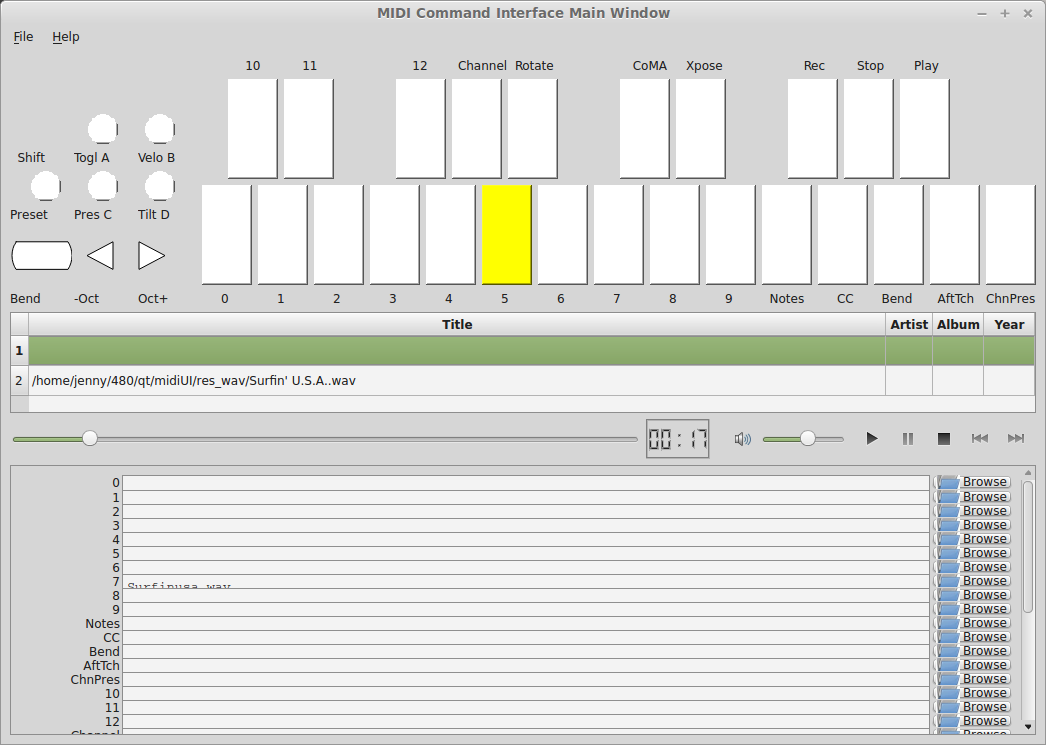
\includegraphics[width=.9\linewidth]{./pic/Screenshot_from_2015-05-04_13:42:14.png}
\end{itemize}

\section{update 4/28/2015, Tuesday}
\label{sec-7}
\subsection{updates}
\label{sec-7-1}
\begin{itemize}
\item Didn't do much code at all, but rather implementing some examples that could help me a little bit. 
\begin{itemize}
\item QMutex, QReadWriteLock, consumer-producer problems seem straight forward to me now;
\item The Mandelbrotset example I typed all the codes from some pic, made them to compile, but I have not got the expected GUI running resuluts yet. I will need to spend some time on it to digest the threads render/insertion/connection and events mechanism.
\item Potentially if possible, I will also need to look into custom designed events, and then postEvents using some other widgets\ldots{}.
\end{itemize}
\item The suggestions I got from the advisor last week, open() and close() the midi device only once, and then define 2 threads (read from \& write to), set up threads communications. These ideas was digested by me already, but the parts I am still not into include:
\begin{itemize}
\item When I have mainwindow.h and mainwindow.cpp using widgets to design the layout, in the main program, when I need to access the individual widgets, like the bottom 15 QPushButtons, how would access these widgets so that I could paint them to different colors to indicate the corresponsive midi controller key is pushed, and playing some song? 
\begin{itemize}
\item When the advisor suggested that I could always declared the data global just like I would define file descriptor to be global and protect the global using mutex, I complained that if I pack the top \& bottom 15 keys into one thread, and pack the bottom configuration area into another thread, then in my GUI for mainwindow.h and mainwindow.cpp, how could I combine them again into a complete gui?\ldots{}.When the advisor hint a little bit more, suddenly I realize that the \textbf{global data structures} (like arrays, whatever\textasciitilde{}) I used can be served as bridge between "front-end" GUI and "back-end" threads\ldots{}.now the project truns out to be straight-forward to me now\ldots{}.
\end{itemize}
\end{itemize}
\item Works needs to do: 
\begin{itemize}
\item phonon play signals \& slots;
\item Threads communications;
\end{itemize}
\item Potential work I am still interested:
\begin{itemize}
\item I used Qt 5.3 before, but then changed back to 4.8.x for phonon use propose only. Together with Fall 2014 semester \textbf{cs480 Senior Design} GUI implementation, I have always been using the old style designs; And I have NOT look into the Qt UIC designer, Qt Quick etc slightly new designed methods. But I am still interested in these parts of knowledge.
\item When this project the most basic implementations are done, I would like to reinstall my Qt and try these new methods once, and to compare both methods to see what I would feel trying the new methods out (before my cs480 Senior Design previous teammates get graduated\ldots{}.:)\ldots{}. 
\begin{itemize}
\item The advisor agreed and reminded me it would means more work ofr me, but I look forward to see what I would feel when I \textbf{really} applied \textbf{fashionable} methods, like xml Qt Quick\ldots{}.
\end{itemize}
\end{itemize}
\end{itemize}
\subsection{Other}
\label{sec-7-2}
\begin{itemize}
\item Finished my \textbf{Change of Study Plan form}, added 30 credits for a M.S. Computer Science, waiting for major advisor to approve it so that I could graduate as planned.
\begin{itemize}
\item I made those changes before 2:00pm yesterday, and the emails were sent out at around 14:15, the advisor would need some time to process his emails, and he agreed that once he gets it approved, I would be able to apply for graduation in Aug, 2015.
\end{itemize}
\item Today when the advisor approved it, submit my application for graduation in Summer (graduate by 8/7/2015, from the I-20) by 4/30/2015.
\item Discuss summer project plan with advisor if possible.
\begin{itemize}
\item The advisor has his followed meeting, so I have NOT been able to do that yet. But I will try to finish the project as musch as possible during this week, and hope to be able to discuss it during coming week's meeting.
\end{itemize}
\end{itemize}

\section{update 4/24/2015, git practise}
\label{sec-8}
\begin{itemize}
\item on 4/7/2015 update, I was supposed to manually resolve conflicts, but I was not aware the problem enough to pay attention to it, ended up by having made three commits; (the readme.org file)
\item And last week Tuesday update I had been blocked by some time becuase of a >100MB pdf file, could use git rm --cached filename;
\item After having spent couple of hours on git docs, began to understand that git branches are well-designed theories, add/delete branches, switch merge/rebase branches, fast-forward, solve conflicts, cherry-pick, set tags, merge/devide commits, etc.
\item Pay careful attention to branch rebase. Do NOT rebase branch after having pushed the necessary updates into remote repository already! Otherwise, it will confuse the whole team who share the repository/project.
\item Added a dev branch for long-term development propose, will add topic or hotfix branches later on when necessary for temporatory bug fix. Try to maintain branches in a professional habit and manner.
\end{itemize}

\section{update 4/21/2015, Tuesday}
\label{sec-9}
\subsection{updates}
\label{sec-9-1}
\begin{itemize}
\item Pretty much all the updates during the past week are included in previous couple of updates, will write advisor review later after meeting though.
\item The followed steps include: 
\begin{itemize}
\item Figure out thread communications. It should be the best method to separate checking midi port task into a thread as I have done before, but need to insert/connect slot thread to be "\textbf{child} " thread maybe (which means move the main function threads part into checking midi port thread)? I want to practise some examples before I code this;
\item Phonon player part try to make play/pause/stop actions responsive first, other stuff, like music table to show music names, previous/next song names are not as important now;
\item Though for Phonon the music table interface update need some work as well. the text book has QxxxTableItem class, and update interface example for references after I get main issues done.
\end{itemize}
\end{itemize}
\subsection{other}
\label{sec-9-2}
\begin{itemize}
\item Review suggestions: After I explained that reading from and write to midi port are designed to be two separated threads (together with either from phonon or timer for LED on time, then write LED off), and supposedly should have QMutex atomic access control, the advisor suggested to open() and close() the device once only (it should be in main program then) and declare the fd = open(DEVICE, O$_{\text{RDWR}}$\ldots{}.) to be global;
\item Need to schedule a time this week ask the advisor to help review "Study Plan", so that I can apply for graduation and get graduated as planed. There was process flow error, and I will need to contact office of registar before I ask for advisor's approvement. Will go to the office afterwards and try to make it work today, get advisor's approvement latest by this Friday.
\item updated late cause I forgot there were two large files more than 100MB, which commits was failed before review.
\end{itemize}

\section{update 4/19/2015}
\label{sec-10}
\begin{itemize}
\item Understand main UI got frozen because checking midi port is time-consuming (count from 0 to 100, 2, whatever\textasciitilde{}!), spent limited time simply tried to apply same threading method on this Dummy class, but failed, I will need to think about it.
\item Still lots of work to do, slot functiona about phonon player, and midi read/write, and potentially more threading as well to make it responsive. Will put more effort on this project for the following several weeks.
\end{itemize}
\section{update 4/18/2015}
\label{sec-11}
\begin{itemize}
\item Separated checking midi port \& corresponding slot function executing in another thread successfully, but mainwindow got blocked from showing up on time, need to find a way to solve this;
\item Still need to work on the slot function for playing audio source files
\end{itemize}

\section{update 4/17/2015}
\label{sec-12}
\begin{itemize}
\item Just understand main thread, and sub-thread signals-slot relationships slightly better by implementing necessary examples
\item want to google and read more docs before my trial of coding\ldots{}.
\item Will still need to work on my codes tomorrow
\end{itemize}

\section{update 4/14/2015}
\label{sec-13}
\subsection{updates}
\label{sec-13-1}
\begin{itemize}
\item Tested the Phonon mediaObject audioOutput process flow is working properly, and the not able to play after having added mediaSource from a thread is caused by the thread, which means it is rather a thread-signal-slot combining/connection problem, rather than Phonon mediaObject audioOutput process flow one;
\item At this point, I still don't have any clear feather idea to solve this problem yet, but together with the idea I presented to the advisor last week, there are several aspect I can try to work on:
\begin{itemize}
\item 1. Try to understand Qt signal-slot connection mechanism deeper and better, the fifth parameter of QObject::connect() has several different types, Qt::QueuedConnection, direct, auto, and implicit sharing;
\item 2. Need to understand through code implementation the most important concepts of "thread safe" and "re-entrant", together with thread-signal-slot implicit sharing mechanism, where could be possibly wrong or potentially affect my current implementation?
\item 3. After above two steps, I believe I would NOT be blinded-trying any more, start to pack Phonon media-related into one thread as I had thought about it before last week's review;
\item 4. And for step 2, one major area that I have not really look into and tried is about eventloop, how to control minor events, especially when multiple threads, QueuedConnection type. This could be a minor aspect of 2.
\item 5. One more trial could conduct on "Serial Communications", not sure if I have translated it correctly. Just like I have "borrowed" some codes from internet about Phonon and made me be able to focus on this dammit thread hell, maybe I could learn from some examples, like how they design and implement when they need audit a port, read from and write to somewhere, one linux example was found in \url{http://mobile.51cto.com/symbian-270754.htm}, will try to copy/paste/test locally and digest and apply if it's helpful.
\end{itemize}
\item That's all the things I have so far, since I have barely made any progress and it is really something interesting, I will work on them this Friday and Saturday, and will update this repository when it's convenient for me for version control among different trials.
\end{itemize}
\subsection{other}
\label{sec-13-2}
\begin{itemize}
\item This morning, I was 10 minutes late, when I set up my computer in CSAC and wrote to the advisor, it was 10:12am already; And it happened that the advisor didn't reply email and didn't show up in his office as well;
\item For last week's meeting, the advisor wrote email that he will be slightly late, but when he show up in CSAC, it was later than 10:40am already, and that's reason I forgot to update the repository before the review;
\item For this spring semester, besides check my codes for details when he wanted, I don't remember if the advisor has offered any constructive suggestions except having asked to open() and close() device each time to see if it could be responsive from different threads on 3/24/2015, while we haven't meet many times neither yet\ldots{}.
\end{itemize}
\subsubsection{Meeting$_{\text{4}}$/7/2015}
\label{sec-13-2-1}
(me\textasciitilde{}) ((me\textasciitilde{})@uxxxx.edu)
Sent:        Tuesday, April 07, 2015 9:25 AM
To:        
(advisor) (advisor@uxxxx.edu)
Hi Dr. Advisor, 

I am in CSAC. When you have your meeting done, or when you are ready, please find me in CSAC.

See you soon\textasciitilde{}!

Thanks,
(me\textasciitilde{})
\subsubsection{Re: Meeting$_{\text{4}}$/7/2015}
\label{sec-13-2-2}
(advisor) (advisor@uxxxx.edu)
You replied on 4/7/2015 10:40 AM.
Sent:        Tuesday, April 07, 2015 9:56 AM
To:        
(me\textasciitilde{}) ((me\textasciitilde{})@uxxxx.edu)
Hi (me\textasciitilde{}) - 

Will be there shortly.

\begin{itemize}
\item advisor
\end{itemize}
\subsubsection{Re: Meeting$_{\text{4}}$/7/2015}
\label{sec-13-2-3}
(me\textasciitilde{}) ((me\textasciitilde{})@uxxxx.edu)
You replied on 4/14/2015 10:12 AM.
Sent:        Tuesday, April 07, 2015 10:40 AM
To:        
(advisor) (advisor@uxxxx.edu)
Sure see you soon.
\subsubsection{Meeting$_{\text{4}}$/14/2015}
\label{sec-13-2-4}
(me\textasciitilde{}) ((me\textasciitilde{})@uxxxx.edu)
Sent:        Tuesday, April 14, 2015 10:12 AM
To:        
(advisor) (advisor@uxxxx.edu)
Dr. Advisor, 

Sorry I was slightly late today. I am in CSAC now and all set up now. When you are ready, please come and find me sitting in previous sit there. 

Thanks,
(me\textasciitilde{})

\section{updates 4/7/2015}
\label{sec-14}
\subsection{updates}
\label{sec-14-1}
\begin{itemize}
\item Googled and reviewed and understood the process flow how Phonon works in Linux environment, but the Phonon MediaObject->play() failed to work properly with separated checking port thread. 
\begin{itemize}
\item To make sure that my understanding and modifications are correct by removing "addFiles" options, I could try old style irresponsive signal-slots just to make sure MediaObject flowchart is correct (have not tried this yet, just know with existing thread, not work);
\end{itemize}
\item Still stuggling with big-picture organization, tried: 
\begin{itemize}
\item separate the checking port tasks into a separate thread, but failed to make Phonon MediaObject->play();
\item separate the checking port tasks into a separate QObject descendant, but still failed to make it work;
\item One more option that I can try would be separate the Phonon media player into a a separate QObject descendant, and together with checking port separate QObject descendant, connecting signals and slots correctly, could be a potential solution, but need separate the Phonon media player first;
\item Hope I can get some help from the advisor as well. The advisor would help look into Qt Creator documents, and I need to google more and implement and test all the limited ideas that I have so far\ldots{}.
\end{itemize}
\end{itemize}
\subsection{other}
\label{sec-14-2}
\begin{itemize}
\item Last week's meeting was cancelled by me because of sickness. It was 3/27 evening when the temperature got extremely low 62F and I hadn't paid any attention to the temperature, and I easily caught cold, got headache and running nose for all these days\ldots{}.
\end{itemize}

\section{update 3/24/2015,}
\label{sec-15}
\begin{itemize}
\item This week's meeting was cancelled, struggling all my way out for "\textbf{H1B sponsorship before 4/1/2015}"\ldots{}\ldots{}
\end{itemize}
\section{Update 3/10/2015, updates include}
\label{sec-16}
\begin{itemize}
\item Current GUI snapshot:
\end{itemize}

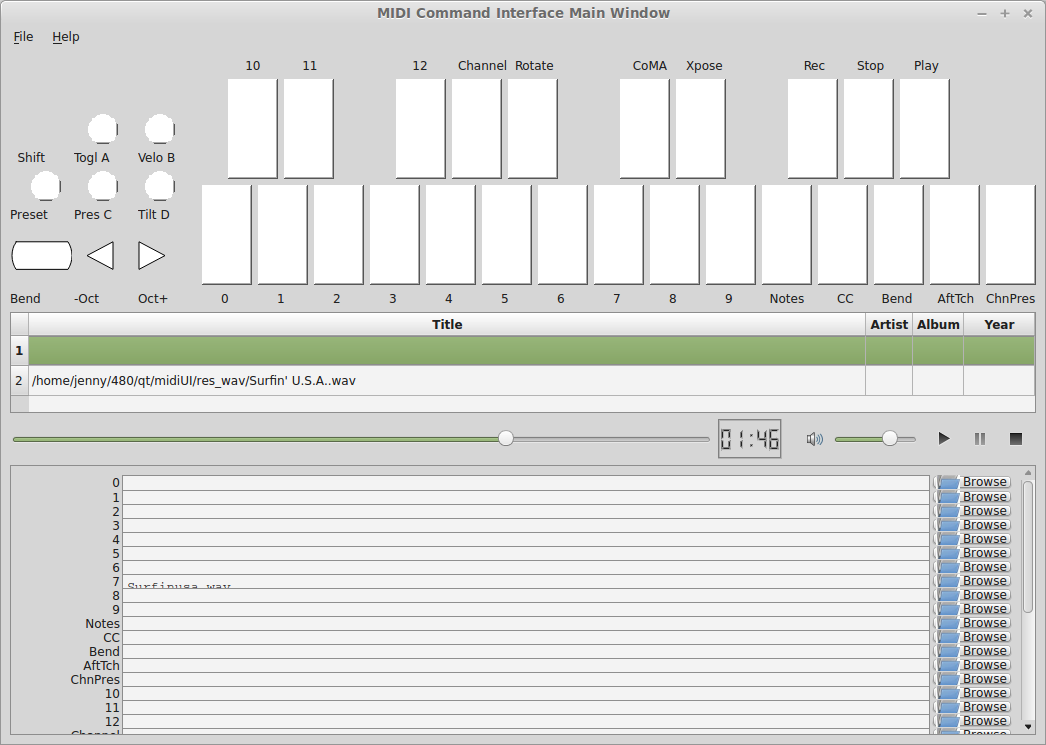
\includegraphics[width=.9\linewidth]{./pic/Screenshot_from_2015-03-08_13:31:00.png}
\subsection{updates}
\label{sec-16-1}
\begin{itemize}
\item On the thread side, I just simply separate the detecting reading from Midi work into a thread, and connected the thread's signals with mainwindow slot function, and this makes the play and stop 100\% responsive already.
\item Then I tried to light LED on for MIdi keys that I have pressed, and the LED on/off was not as repsonsive as I expected, would look into this later on;
\item exchanged QSound with phonon module to satisfy my advisor's new increased requirements during last review meeting.
\item Phonon module is fully-functional by down-grading qt Creator from 5.3.x to 4.8.6 version and install phonon module, just need some extra work to fix minor bugs and satisfy the advisor's requirements (while I kept some buttons and toolbars and codes just for my debugging propose and convenience only, I could easily remove them later on according to the advisor's suggestions);
\end{itemize}
\subsection{other}
\label{sec-16-2}
\begin{itemize}
\item Last week my advisor complained that the hour I showed him too much code, he doesn't want to look into code that much yet. And he would rather help me with threads communications.
\item After all my possible demos by commenting some codes out, even with threads, my advisor didn't offer any constructive suggestions. Gosh, I missed the mentor so much, who as the technical lead knows programs and projects great, inspired and taught me sincerely and effectively during the internship season\ldots{}.
\item For this week's meeting, I am going to set my laptop into CSAC, so that I don't have to put everything on my knees and not formal and convenient at all.
\item Since my advisor doesn't want to review my codes, even he specificly checked for detail how I declared and initialized my playthread in my mainwindow.cpp file during last review meeting. Since I need to get graduated any way, and I have always been blocked and I have not set up the online full study plan yet, I would need to \textbf{discuss the graduation date and process} with my advisor today if I have any extra time.
\item The advisor sent email saying that he will be slightly late for today's meeting.
\end{itemize}
\subsection{Last week's meeting explain}
\label{sec-16-3}
Last week's weekly meeting was cancelled by advisor, emails are attached below;

\subsubsection{No meeting today?}
\label{sec-16-3-1}
(my advisor)@gmail.com [(my advisor)@gmail.com] on behalf of (my advisor) [(my advisor)@xxxxx.uxxxxx.edu]
You replied on 3/3/2015 9:47 AM.
Sent:        Tuesday, March 03, 2015 9:12 AM
To:        (me\textasciitilde{}~) ((me\textasciitilde{}~)@vandals.uxxxxx.edu)

Hi (me\textasciitilde{}~) - 

I have a deadline today - would it be possible to meet on thursday, 10:00 instead of today?

Thanks!

\begin{itemize}
\item (my advisor)
\end{itemize}
\subsubsection{RE: No meeting today?}
\label{sec-16-3-2}
(me\textasciitilde{}~) ((me\textasciitilde{}~)@vandals.uxxxxx.edu)
Sent:        Tuesday, March 03, 2015 9:47 AM
To:        
(my advisor) [(my advisor)@xxxxx.uxxxxx.edu]
Hi Dr. (My Advisor), 

Yes let's meet on Thursday 10:00am then. I will write to you if I have any conflict on that time if there is any by then (so far no conflicts). 

(explain: The reason I wrote this way was that I have short chats with recruitors on Tuesday and Wednesday, and there is NO reason that I should NOT put my job hunting for H1B sponshorship as my first priority. If I would have phone screen on Thursday, I don't want to it be blocked by the weekly review.)

Thanks,
(me\textasciitilde{}~)
\subsubsection{Can't meet today}
\label{sec-16-3-3}
(my advisor)@gmail.com [(my advisor)@gmail.com] on behalf of (my advisor) [(my advisor)@xxxxx.uxxxxx.edu]
Sent:        Thursday, March 05, 2015 7:31 AM
To:        
Huang, (me\textasciitilde{}~) ((me\textasciitilde{}~)@vandals.uxxxxx.edu)
Hi (me\textasciitilde{}~) - 

I just realized that I have a thesis defense today at 9:30, so I can't meet today. Let's shoot for our regular time next week.

(explain: I guess my advisor simply forgot either my weekly review scheduled by himeself two days ago, or he simply forgot the student's defense which one he was interested. No problem with me at all. )

\begin{itemize}
\item (my advisor)
\end{itemize}
\subsection{review resuluts}
\label{sec-16-4}
\begin{itemize}
\item The advisor came to CSAC at 10:26am, and we did have about half an hour meeting before his 11:00am meeting.
\item For the phonon GUI, except the musicTable and menubar, we agreed that we will keep all the necessary informations including seekslider, timerLCD, volumeSlider, play/pause/stop buttongs;
\item I am asked to follow with midi threads controlling LED on/off for the coming half a month. And since I am mainly focusing on my job hunting for this month, it would be ok if I make slow progress or even no progress at all for this month. And since I have done lot's of work during the passed semesters, even the project doesn't work as expected, my advisor agreed that it won't affect my graduation. But I will try my best to make it work.
\item I \textbf{will graduate} as I planned during summer this year.
\item For the followed half a month (coming week is spring break and campus will be closed, no meeting on 3/17/2015) try to make LED on/off responsive;
\item constructive suggestions from the advisor are that try to open() and close() device each time to see if it could be responsive from different threads.
\end{itemize}

\section{update 3/3/2015, meeting canceled for today}
\label{sec-17}
\begin{itemize}
\item The meeting was cancelled for today, will update some other day when this week's schedule get fixed.
\end{itemize}
\section{update 2/24/2015, updates include}
\label{sec-18}
\subsection{updates}
\label{sec-18-1}
\begin{itemize}
\item idol(3); moved to the correct position to paint GUI button responsively;
\item modified "Play" key to be "Stop" playing a music key, set upper row last key as "STOP" key;
\item made playing a song and stop the song become responsive (two operations in total) by implementing play the song through a thread; This way the "STOP" key could work;
\item Issue is that only 2 operations responsive, but need to be always responsive. The reason for this failed could be playing thread didn't reinitialize as expected, or need another thread to always check midi user input, and I suspect the reason is more likely the latter; So moved to remove main GUI clicks step and use midi as the main input;
\item I mean to use while loop, but even after the advisor approved the method, afterwards I realized that multi-threading is the more intuitive and correct way to do it, so skipped while loops;
\item I packed my data array buffer into an object and include setter/getter; I should have read thread always checking midi input periodically; I should have write thread to write back to midi to light LED on; I was blocked slightly when finished reading but not implementing writing, I failed to read the data needed to play the song; will try this appoarch later;
\item After get blocked using reading thread, I changed back to the advisor suggested using while loop way. As predicted, the main UI got blocked by the while loop, which still point/approve to the multi-threading appoarch;
\item This is the first time that I realize such blocking problems, though I made quite some progress, and last week's meet suggestions/updates is NOT for one week to finish, rather eventual goals, so I am confident that eventually I would get all these problems solved;
\item The write back to midi to light LED on for the key pressed, and methods are ready there already, I just need to make my threads work first, then use a thread to write back to midi when necessary,
\end{itemize}
\subsection{other}
\label{sec-18-2}
\begin{itemize}
\item As listed above, review the play/stop details and issues, reading thread issues, and while loop issues sequencially and logically with advisor by demo all these different version, and show necessary codes parts;
\item The project goal keeps the same, and the advisor actually maybe interested in "PAUSE" button and seekslider bar, and later if I have time, would work on that;
\item For the followed several weeks, try to get a responsive softwares in fairly reasonable period.
\end{itemize}

\section{Update 2/19/2014, updates include}
\label{sec-19}
\subsection{updates}
\label{sec-19-1}
\begin{itemize}
\item These are two sets in the MIDI keyboard, the 25 key main board, and the adjustment 8 keys;
\item Corresponded the main keyboard keys with the same "surfinUSA.wav" song, and it works;
\item Tested that all the 25 keys (I tested 4-5 keys by random sample) bonds to one song as a comand controller should work;
\item Applied the same method on the left side 8 keys, but they are completely different set, so need further look into the sets ("Bend" could show key values, but the value could be changed to, and the other seven could NOT print Note ON/OFF values cause they are functionally different);
\item GUI Interface keeps the same unchanged, so refer to last update for interface snapshot;
\item I have spent tons of hours on Emacs ever since Fall 2012 triggered by Emacs Lisp program hightlights, and I still got blocked by unexpected bugs from time to time, but still, have been blocked by thousands of times, I still like Emacs the most. Fully functional Emacs without bugs significantly improves efficiency for me. Now brought readme.tex and readme.pdf back, I like to have them before git update to avoid multiple unnecessary updates\ldots{}
\end{itemize}
\subsection{todo}
\label{sec-19-2}
\begin{itemize}
\item So far linked to only one song, I have about 4-5, and need to link all of them to the keys (instead of link all the keys to the same song);
\item Add two buttons for "Pause" and "Stop" in GUI to pause/stop playing a song;
\item To light the midi controller LED on while the specific key pressed and light it on during the song time;
\item Two set of input, midi controller and GUI buttons, prefer midi controller for input during tower show; The advisor said use an infinte loop for Checking midi input is ok, but I (me\textasciitilde{}) would expect to explore qt threads when loop is functional; The advisor expect that the midi controller should be responsive, so I should program to update midi-readin frequently (maybe even less than 500 ms interval according to the advisor);
\item Though "the more information the better", the sliderbar is not necessary, I will list it as low priority.
\item These are the suggestions that the advisor offered during morning meeting, and before the followed week meeting, I will try to finish as much as I can.
\end{itemize}
\subsection{other issues}
\label{sec-19-3}
\begin{itemize}
\item The advisor and I rescheduled our meeting time to be 2:30pm on Wednesday afternoon because actually he has bi-weekly meeting at the original meeting time;
\item Then I realize that I failed to state it clear that I need to work at 3pm means I needs to be well uniformly-dressed and be able to clock in and start work immediately, so we will have only about 15 minutes, and even advisor says I may start early, but I don't want to run to work late at times.
\item I wrote to the advisor and during yesterday's short meet we rescheduled the meeting time to be "\textbf{10:00am - 11:00am on Tuesday}" and for this week's meeting rescheduled to be this morning at 8:30am - 9:30am (the advisor showed up at 9:05, so we did have about half an hour meeting this morning. He had visitor at 9:30am).
\item Later on will update this repository weekly \textbf{around 11:00am within +/- 30 minutes} time period to help and enforce myself to make some progress weekly.
\end{itemize}

\section{Update 2/12/2014, updates include}
\label{sec-20}
\subsection{updates}
\label{sec-20-1}
\begin{itemize}
\item Didn't start until this week was mainly before the foot court work had waited more than one week to get docs processed, and waiting for work Schedule before Scheduling with advisor, and advisor approved it.
\item Scheduled Wednesday 12:30-1:30pm to meet advisor weekly, and will update at least once a week to record progress.
\item For coming week's meeting, advisor suggested to get more keys combines with songs in the normal 25 key set besides the finished one.
\item Today got the Rectangle/Triangle shapes work and ready.
\end{itemize}
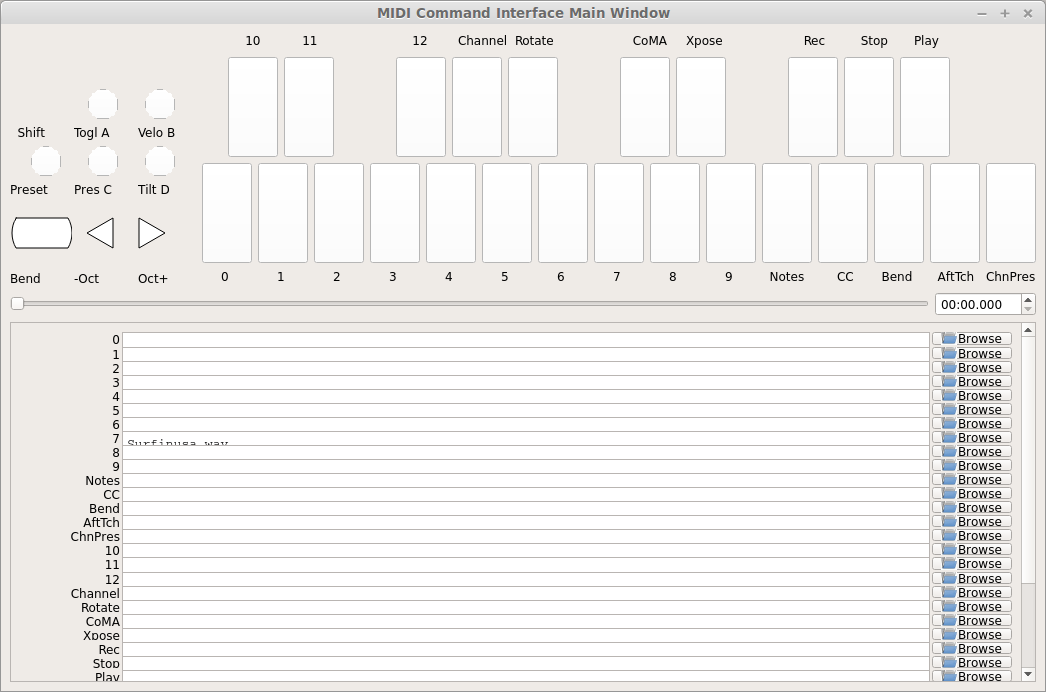
\includegraphics[width=.9\linewidth]{./pic/Screenshot_from_2015-02-13_22:19:11.png}

\section{Update 12/11/2014, updates include}
\label{sec-21}
\subsection{updates}
\label{sec-21-1}
\begin{itemize}
\item Temporatorily mimic phonon seekslider, but have not connected the signals and slots fully functioning yet;
\item This seekslider may still eventually came back to use Phonon library using Qt4.8 version;
\item So far consider this as a bonus feature;
\end{itemize}
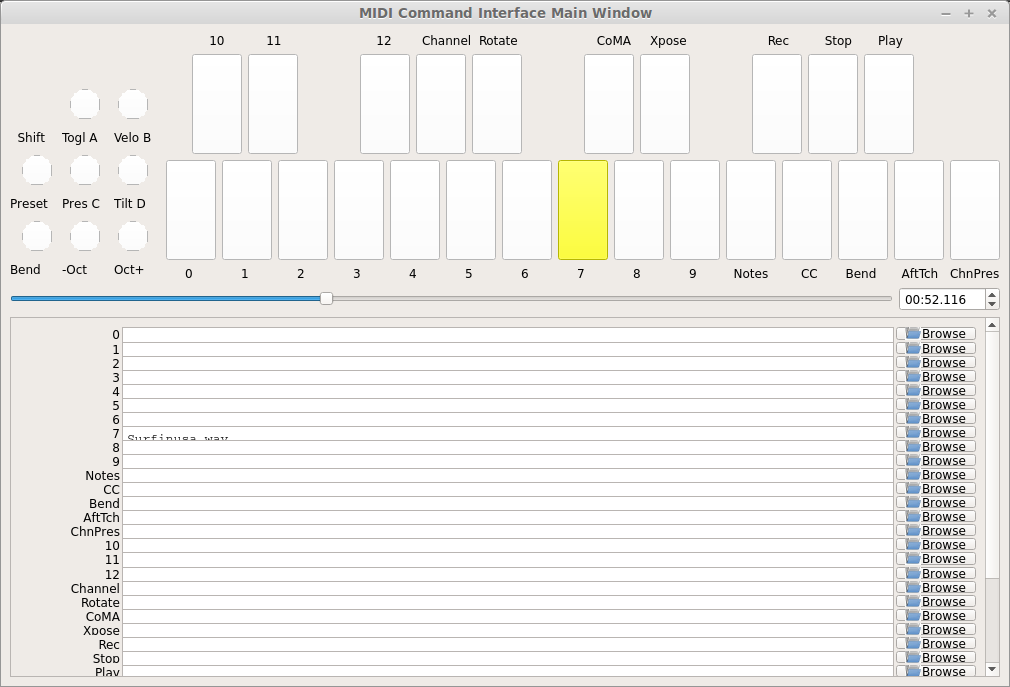
\includegraphics[width=.9\linewidth]{./pic/Screenshot_from_2014-12-11_17:34:24.png}
\subsection{review}
\label{sec-21-2}
\begin{itemize}
\item Because of lack Xbee modules (needs devices from intstructor), so far playing only .wav file is ok;
\item It is basic, setting one buttone to work only, without any threads yet, but will expend it to be better during spring semester.
\item Spring semester (1 credit) will pack all my instructor's Tower Play modules into a well-designed fully-functional softwares for user's convenience.
\end{itemize}
\section{Update 12/09/2014, updates include}
\label{sec-22}
\begin{itemize}
\item worked in it a little bit to set the connections between Midi controller and Qt Creator;
\item tried to implement pthead for reading user input, but got slightly frustrated today, and applied easier methods instead;
\item the project basically satisfied the instructor's requirements for connecting one key to work for playing his sequence, for example, Surfinusa.wav file;
\item Will demo to his to see if he has better suggestions.
\end{itemize}
\section{Update 11/23/2014, updates include}
\label{sec-23}
\begin{itemize}
\item Cleaned repository so that it looks clean and nice;
\item Remove menubar as suggested by advisor;
\item Removed topright four line texts cause it's not necessary;
\item Shifted top line keys so that they look like original midi controller layout;
\item Changed PlainTextEdit so that they satifies the requirements;
\item Added left side 8 keys, just that three keys \textbf{Bend}, \textbf{-Oct}, \textbf{Oct+} are \textbf{NOT} like the original shapes yet, need work on them later on;
\item Will link possible functionalities to make it a functional softwares first, and then updates minus issues.
\item Current layout looks as below snapshotted:
\end{itemize}

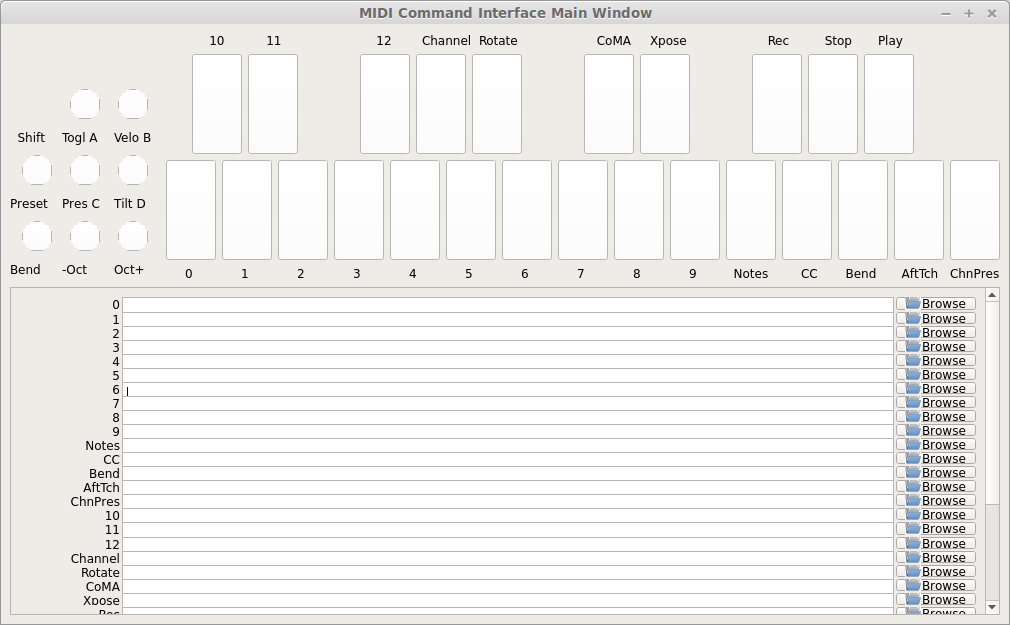
\includegraphics[width=.9\linewidth]{./pic/Screenshot_from_2014-11-23_13:20:06.png}  
\section{Review 11/21/2014, updates include}
\label{sec-24}
\subsection{Review Contents}
\label{sec-24-1}
\begin{itemize}
\item Created most basic interface for the client, and reviewed with course instructor.
\item Demo the most basic interface to him, and get corresponding specific requirements as listed followed.
\end{itemize}

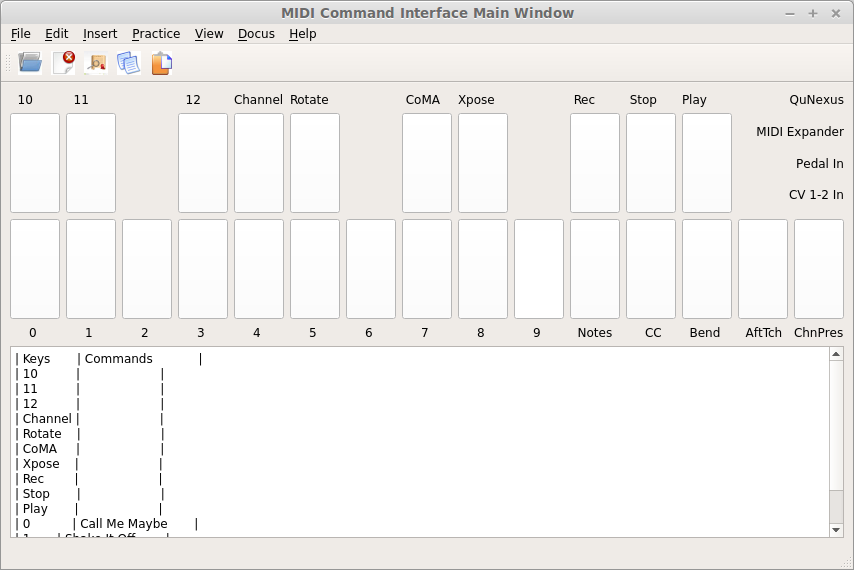
\includegraphics[width=.9\linewidth]{./pic/2014-11-20_21:52:19.png}
\subsection{Detailed Requirements}
\label{sec-24-2}
\begin{itemize}
\item menubar is NOT necessary, and could be removed away;
\item Interface topright four line texts are not necessary, could be removed away;
\item Interface top line keys should shift to the right by half key width so that the interface looks similar to the original midi controller keyboard;
\item PlainTextEdit should be changed to be array of 25/33 lines of (text label, file name editor, browse QPushButton keys) layout;
\item Left handside 8 keys should be included in the midi interface even functionalities are not required at this moment;
\item When finished the above basic ones, if I have extra time, could explore the left side 8 keys to test if it is possible to use them to set a bunch of sequence so that save time when needed compared with set sequence one by one from the basic 25 keys.
\end{itemize}
\section{Project Requirements}
\label{sec-25}
\begin{itemize}
\item Use QuNexus Midi controller as a command controller to manipulate play sequence for tower lights show;
\item Besides the main functionalities, create a Qt Creator Interface to help facilate the tower light playing process for clients convenience.
\end{itemize}
\section{main functionality}
\label{sec-26}
\subsection{Read data from MIDI}
\label{sec-26-1}
\begin{itemize}
\item Use the MIDI Controller as a speical Controller that can be operated to play specific songs sequence, or do some specific work.
\item play specific sequence may be the work for keys 0-9, and 10-12, how about other 20 keys? Do they require specific work to be done?
\end{itemize}
\subsection{Write data back to MIDI}
\label{sec-26-2}
\begin{itemize}
\item When a key was pushed, the specific Controller key's LED is supposed to be on to indicate the operation.
\item Trick about the LED to be continuously on is that when a key is pressed, that is 1 byte that indicates the "Duration" of the key press, I may need to 
\begin{itemize}
\item try to set this byte to be a large value, (1 byte, 2$^{\text{8}}$ = 256, it has limits!)
\item or continuously reset is to be that large value;
\item or continuously write this key to be pressed data back to MIDI with time intervals
\end{itemize}
\end{itemize}
\section{Programming Language}
\label{sec-27}
\subsection{Qt}
\label{sec-27-1}
\begin{itemize}
\item the worries that I have by using Qt is that if Qt has the capability to handle the MIDI-Linux connection problems.
\item And also Qt-to-Audio (linux) connection things as well. Should it be Qt, or as far as I can set it to work in Linux, just let it be that way then?
\end{itemize}
\subsection{c++}
\label{sec-27-2}
\begin{itemize}
\item I believe C++ is the most widely used Language used by those midi sequencer softwares, so I have no better choice than c++ right now.
\end{itemize}
\section{Interface Design}
\label{sec-28}
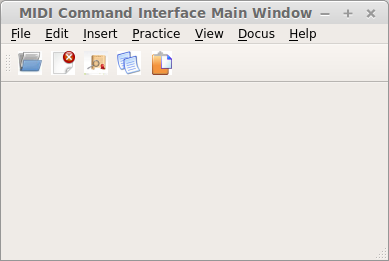
\includegraphics[width=.9\linewidth]{./pic/menu.png}

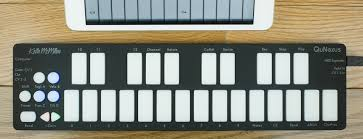
\includegraphics[width=.9\linewidth]{./pic/midi.jpg}
\section{Midi keys and corresponded operations}
\label{sec-29}
\begin{table}[htb]
\caption{midi keys and corresponded operations}
\centering
\begin{tabular}{ll}
\hline
Keys & Commands\\
\hline
10 & \\
11 & \\
12 & \\
channel & \\
Rotate & \\
CoMA & \\
Xpose & \\
Rec & \\
Stop & \\
Play & \\
\hline
0 & Call Me Maybe\\
1 & Shake It Off\\
2 & All About That Bass\\
3 & \ldots{}\\
4 & \\
5 & \\
6 & \\
7 & \\
8 & \\
9 & \\
\hline
Notes: & \\
CC & \\
Bend & \\
AftTch & \\
ChnPres & \\
\hline
Togl A & \\
Velo B & \\
Preset & \\
Pres C & \\
Tilt D & \\
Bend & \\
Oct- & \\
Oct+ & \\
\hline
\end{tabular}
\end{table}
\section{Interface Guide}
\label{sec-30}
\begin{itemize}
\item Give text instructions on how to use the Interface, and what are the corresponded operations by press specific keys.
\item Like list the above table in the Interface Guide text area.
\end{itemize}
\section{References}
\label{sec-31}
\subsection{For circle QPushButton}
\label{sec-31-1}
\begin{itemize}
\item \url{http://stackoverflow.com/questions/12734319/change-rectangular-qt-button-to-round}
\end{itemize}
\subsection{Draw circle separate}
\label{sec-31-2}
\begin{itemize}
\item \url{https://coderalbert.wordpress.com/2014/03/16/creating-circle-in-linux-using-qt-creator/}
\end{itemize}
\subsection{For Rectangle Arc}
\label{sec-31-3}
\begin{itemize}
\item \url{http://stackoverflow.com/questions/20416789/how-to-add-a-small-triangle-at-one-of-the-corners-of-qwidget}
\end{itemize}
\subsection{PaintEvent Triangle}
\label{sec-31-4}
\begin{itemize}
\item \url{http://stackoverflow.com/questions/20416789/how-to-add-a-small-triangle-at-one-of-the-corners-of-qwidget}
\item \url{http://stackoverflow.com/questions/3894737/qt4-how-to-draw-inside-a-widget}
\item \url{http://qt-project.org/forums/viewthread/1623}
\item \url{http://stackoverflow.com/questions/7968269/basic-qt-gui-qpushbutton-for-drawing-a-line}
\end{itemize}
\subsection{QPushButton::drawButton(QPainter *painter);}
\label{sec-31-5}
\begin{itemize}
\item \url{https://www.tbi.univie.ac.at/~pmg/tutorials/QT/html/qpushbutton.html}
\end{itemize}
\subsection{QGraphicsSene QGraphicsProxy\ldots{}}
\label{sec-31-6}
\begin{itemize}
\item \url{http://qt-project.org/forums/viewthread/4020}
\end{itemize}
\subsection{QPushButton raised enabled}
\label{sec-31-7}
\begin{itemize}
\item \url{http://www.qtcentre.org/threads/42852-QStyledItemDelegate-paint-QPushButton-with-stylesheet}
\end{itemize}
\subsection{QPushButton two icons}
\label{sec-31-8}
\begin{itemize}
\item \url{http://www.qtcentre.org/threads/39445-How-to-add-two-icons-images-to-the-same-QPushButton}
\end{itemize}
\subsection{QPainter}
\label{sec-31-9}
\begin{itemize}
\item \url{http://qt-project.org/forums/viewthread/23628}
\end{itemize}
\subsection{QGridLayout ScrollArea}
\label{sec-31-10}
\begin{itemize}
\item \url{http://qt-project.org/forums/viewthread/20843}
\item \url{http://qt-project.org/forums/viewthread/20924/}
\end{itemize}
\subsection{Linux Midi}
\label{sec-31-11}
\begin{itemize}
\item \url{https://ccrma.stanford.edu/~craig/articles/linuxmidi/input/section1.html}
\item \url{https://ccrma.stanford.edu/~craig/articles/linuxmidi/}
\end{itemize}
\subsection{Open device}
\label{sec-31-12}
\begin{itemize}
\item \url{http://pubs.opengroup.org/onlinepubs/009695399/functions/open.html}
\end{itemize}
\subsection{Qt QIODevice}
\label{sec-31-13}
\begin{itemize}
\item \url{http://doc.qt.digia.com/qq/qq12-iodevice.html}
\item \url{http://stackoverflow.com/questions/14821792/what-does-file-openqiodevicereadonly-mean}
\end{itemize}
\subsection{Qt Debugging}
\label{sec-31-14}
\begin{itemize}
\item \url{https://bbs.archlinux.org/viewtopic.php?id=174523}
\item \url{http://www.qtcentre.org/threads/53549-connect}()-terminates-the-program
\end{itemize}
\subsection{pulseaudio linux mint}
\label{sec-31-15}
\begin{itemize}
\item \url{http://community.linuxmint.com/software/view/pulseaudio}
\lstset{language=c++,label= ,caption= ,numbers=none}
\begin{lstlisting}
towerplayer  ./towerplayer Surfinusa.wav surfinUSA.tan
Loading Surfinusa.wav
File Size=26368316
Header Size=16
Data Size=26368272 (0x1925910)
Done reading tan file!
Checking for fast nodes
unable to open ftdi (xbee) device: -3 (device not found)
\end{lstlisting}
\end{itemize}
\subsection{QSound example}
\label{sec-31-16}
\begin{itemize}
\item \url{http://doc.qt.digia.com/3.3/sound-example.html}
\end{itemize}
\subsection{QSound QSoundEffect(pulseaudio): Error Decoding course}
\label{sec-31-17}
\begin{itemize}
\item \url{https://together.jolla.com/question/53394/qsoundeffectpulseaudio-error-decoding-sourc/}
\end{itemize}
\subsection{QTimer}
\label{sec-31-18}
\begin{itemize}
\item \url{http://qt-project.org/forums/viewthread/27190}
\end{itemize}
\subsection{Triangle}
\label{sec-31-19}
\begin{itemize}
\item \url{http://en.wikibooks.org/wiki/Qt/Qt_Quick_Overview}
\item \url{http://qt-project.org/forums/viewthread/25624}
\item \url{http://stackoverflow.com/questions/24672146/qpainter-draw-lien}
\item \url{http://doc.qt.digia.com/4.6/widgets-styles.html}
\item \url{http://qt-project.org/doc/qt-4.8/painting-painterpaths-window-cpp.htm}
\end{itemize}
\subsection{play loops}
\label{sec-31-20}
\begin{itemize}
\item \url{http://stackoverflow.com/questions/16751778/qt-qsound-looping}
\item \url{http://forum.codecall.net/topic/71902-qt-c-play-sound-on-key-press-stops-working-after-a-few-seconds/}
\end{itemize}
\subsection{Phonon}
\label{sec-31-21}
\begin{itemize}
\item \url{http://tuxradar.com/content/how-it-works-linux-audio-explained}
\item \url{http://bbs.qter.org/forum.php?mod=viewthread&tid=784}
\item seek slider failed: \url{http://pencil-animation.org/forum/viewtopic.php?id=672}
\item \url{http://qt-project.org/doc/qt-4.8/phonon-qmusicplayer.html}
\item \url{http://www.360doc.com/content/12/1110/17/6828497_247047662.shtml}
\item \url{http://max.book118.com/html/2014/0117/5589932.shtm}
\item phonon classsic example: \url{http://doc.qt.digia.com/4.6/phonon-qmusicplayer.html}
\end{itemize}
\subsection{QThread}
\label{sec-31-22}
\begin{itemize}
\item \url{http://www.360doc.com/content/12/0218/20/6828497_187676466.shtml}
\item \url{http://www.360doc.com/content/12/1106/14/7899729_246182251.shtml}
\item \url{http://qt-project.org/wiki/Threads_Events_QObjects_Chinese}
\item \url{http://my.oschina.net/laopiao/blog/88158}
\item example \url{http://blog.csdn.net/small_qch/article/details/6681907}
\item \url{http://www.kuqin.com/qtdocument/threads.html}
\item \url{http://no001.blog.51cto.com/1142339/277004}
\item use \textbf{moveToThread()} to change the affinity. explain example \url{http://stackoverflow.com/questions/15034255/launch-phonon-player-in-a-different-thread}
\item \url{http://stackoverflow.com/questions/4093159/what-is-the-correct-way-to-implement-a-qthread-example-please}
\item \url{http://gotoanswer.com/?q=Qt+Signals+and+slots+in+a+QThread}
\item ����ͨѶ \url{http://mobile.51cto.com/symbian-270754.htm}
\item \url{http://www.xuebuyuan.com/973565.html}
\item \url{http://mobile.51cto.com/symbian-268690.htm}
\item \url{http://mobile.51cto.com/symbian-268690_1.htm}
\item \url{http://mobile.51cto.com/symbian-268360.htm}
\item \url{http://stackoverflow.com/questions/15034255/launch-phonon-player-in-a-different-thread}
\end{itemize}
\subsection{midi read/write separate}
\label{sec-31-23}
\begin{itemize}
\item \url{http://www.alsa-project.org/alsa-doc/alsa-lib/rawmidi.html}
\item seems to be something relative \url{https://github.com/mixedinkey-opensource/MIKMIDI}
\item \url{https://github.com/vishnubob/python-midi}
\end{itemize}
\subsection{volatile}
\label{sec-31-24}
\begin{itemize}
\item \url{http://www.infoq.com/cn/articles/ftf-java-volatile}
\item \url{http://www.blogjava.net/sunzhong/articles/295916.html}
\item \url{http://www.iteye.com/topic/109150}
\item \url{http://blog.csdn.net/zhaoyu_android4311/article/details/8363892}
\item \url{http://www.programgo.com/article/24803476877/}
\item \url{http://wenjun.org/c/952.html}
\item \url{http://www.xuebuyuan.com/1530042.html}
\item \url{http://rock3.info/blog/2013/11/24/linux-c\%E4\%B8\%AD\%E8\%B0\%83\%E7\%94\%A8\%E6\%B1\%87\%E7\%BC\%96\%E7\%94\%A8\%E6\%B3\%95/}
\end{itemize}
% Emacs 24.3.1 (Org mode 8.2.7c)
\end{document}